\chapter{Understanding Conditioned \break Neural Code Models}
\label{ch6:conditioned}

%1. Establishing the importance of the field
The combination of large amounts of freely available code-related data, which can be mined from open source repositories, and ever-more sophisticated Neural Code Model (\nlm) architectures have fueled the development of Software Engineering (SE) tools with increasing effectiveness. \nlms have (seemingly) illustrated promising performance across a range of different SE tasks~\citep{Watson:ICSE20,White:MSR15,ciniselli2021empirical,Mastropaolo2021StudyingTasks}. In particular, \textit{code generation} has been an important area of SE research for decades, enabling tools for downstream tasks such as code completion~\citep{MSR-Completion}, program repair~\citep{Chen2019sequencer}, and test case generation~\citep{Watson:ICSE20}. In addition, industry interest in leveraging \nlms for code generation has also grown as evidenced by tools such as Microsoft's IntelliCode \citep{intellicode}, Tabnine \citep{tabnine}, OpenAI's Codex \citep{openai_codex}, and GitHub's Copilot \citep{github_copilot}. Given the prior popularity of code completion engines within IDEs~\citep{murphy2006ide}, and the pending introduction of, and investment in commercial tools, \nlms for code generation will almost certainly be used to help build production software systems in the near future, if they are not being used already.

%2. Presenting the general problem
However, it is generally accepted that \textit{Neural Language Models} operate in a black-box fashion. That is, we are uncertain how these models \textit{arrive at decisions}, which is why \nlms suffer from \textit{incompleteness} in problem formalization \citep{Doshi-Velez2017TowardsLearning}. As such, much of the work on \nlms has primarily relied upon automated metrics (\eg Accuracy, BLEU, METEOR, ROUGE) as an evaluation standard. Skepticism within the natural language processing (NLP) research community is growing regarding the efficacy of current automated metrics ~\citep{ribeiro2020checklist, rei2020comet, kocmi2021ship}, as they tend to overestimate model performance. Even benchmarks that span multiple tasks and metrics have been shown to lack robustness, leading to incorrect assumptions on model comparisons \citep{dehghani2021benchmark}. 

%3. Previous and/or Current Research
Despite the increasing popularity and apparent effectiveness of neural code generation tools, there is still much that is unknown regarding the practical performance of these models, their ability to learn and predict different code-related concepts, and their current limitations. Some of the most popular models for code generation have been adapted from the field of NLP, and thus may inherit the various limitations often associated with such models --- including biases, memorization, and issues with data inefficiency, to name a few~\citep{bender2021parrots}. In fact, recent work from Chen \etal \citep{chen2021evaluating} illustrates that certain issues, such as alignment failures and biases, do exist for large-scale \nlms. Most of the conclusions from Chen~\etal's study were uncovered through manual analysis, \eg through sourcing counterexamples, making it difficult to rigorously quantify or to systematically apply such an analysis to research prototypes~\citep{wu2019errudite}. Given the rising profile and role that \nlms for code generation play in SE, and the current limitations of adopted evaluation techniques, it is clear that new methods are needed that provide deeper insight into \nlms' performance. Notable work has called for a more systematic approach \citep{ribeiro2020checklist} that aims to understand a given model's behavior according to its linguistic capabilities and tests customized for the given task for which a model is applied.

%4. The GaP (or what is missing). Describe the specific problem. Present a prediction to be tested. 
As the discussion above suggests, while it may appear that \nlms have begun to achieve promising performance, it is clearly insufficient to examine \underline{only} prediction values (\ie the \textit{\textbf{what}} of \nlms' decision). This current status quo, at best, provides an incomplete picture of the limitations and caveats of \nlms for code. %As scientists, we allow theories to be falsifiable by means of empirical observations and proper model explanations to avoid pseudo-scientific claims. 
Given the potential impact and consequence of these models and their resulting applications, there is a clear need to strive for a more complete understanding of how they function in practice. As such, we must push to understand how \nlms arrive at their predictions (\ie the \textit{\textbf{why}} of \nlms' decision). In this paper, we cast this problem of achieving a more complete understanding of \nlms as an \textit{Interpretable Machine Learning} task and posit that we can leverage the theory of \textit{causation} as a mechanism to explain \nlms prediction performance. We hypothesize that this mechanism can serve as a useful debugging tool for detecting biases, understanding limitations, and eventually, increasing the reliability and robustness of \nlms employed for the task of code generation \citep{molnar2019interpret,Doshi-Velez2017TowardsLearning}.

%5.Describing the paper itself
This paper introduces \codegen, a novel post-hoc interpretability method specifically designed for understanding the effectiveness of \nlms. The intention of \codegen is to establish a robust and adaptable methodology for \textit{interpreting} predictions of \nlms trained on code in contrast to simply \textit{measuring} the accuracy of these same \nlms. More specifically, \codegen consists of two major conceptual components, (i) a \textit{structural causal graph}, and (ii) a \textit{causal inference mechanism}. \codegen's \textit{structural causal graph} maps model predictions to programming language (PL) concepts and variations in test datasets at different levels of granularity, thus enabling statistical analyses of model predictions rooted in understandable concepts. While our methodology allows for extensiblility in defining relevant PL concepts, we offer an initial \textit{code taxonomy} as a generalizable example. However, examining statistical properties of model predictions in isolation does not provide \textit{explanations} regarding observed performance. As such, the second theoretical component of \codegen adopts a \textit{causal understanding} mechanism that can explain observed trends in model predictions rooted in the aforementioned programming language concepts. This causal inference mechanism allows for the generation of explanations of model performance rooted in \codegen's understandable concepts. Through the introduction of this interpretability framework, we aim to help SE researchers and practitioners by allowing them to understand the potential limitations of a given model, work towards improving models and datasets based on these limitations, and ultimately make more informed decisions about how to build automated developer tools given a more holistic understanding of \textit{\textbf{what}} \nlms are predicting and \textit{\textbf{why}} the predictions are being made.

%5 Announcing Findings
To showcase the types of insights that \codegen can uncover, we perform a case study on different variations of two popular deep learning architectures for the task of code generation, namely RNNs~\citep{RNNs} and Transformers \citep{vaswani2017transformers} trained on the CodeSearchNet dataset~\citep{husain2019codesearchnet}. We instantiated our study using ten structural code categories derived from the Java programming language. This study resulted in several notable findings illustrating the efficacy of our interpretability technique: (i) we find that our studied models learn to predict tokens related to code blocks (\eg brackets, parentheses, semicolons) more effectively than most other code token types (\eg loops, conditionals, datatypes), (ii) we found that our studied models are sensitive to seemingly subtle changes in code syntax, reinforcing previous studies concluding the same~\citep{rabin2021generalizability}, and (iii) our studied models are only marginally impacted by the presence of comments and bugs, which challenges findings from previous work~\citep{Baishakhi2016buggy}.

%------------------------------------------------

\section{The \codegen Methodology }
\label{sec:approach-conditioned}

This section presents \codegen, a set of causal inference tools to \textit{interpret the prediction performance} of \nlms by connecting causal models to data. \codegen instantiates the concepts and theory discussed in the previous section by introducing three stages (St$_1$-St$_3$): (i) \textit{Modeling Causal Variables}, (ii) \textit{Computing Causal Inference}, and (iii) \textit{Evaluating Causal Effects}. Because \codegen focuses its analysis upon the probability distribution of Next Token Predictions (NTPs) and Cross-Entropy, it falls into the category of model-specific (\ie to \nlms) post-hoc interpretability methods \citep{molnar2019interpret}. We have implemented \codegen in an open source library, which we will make freely available upon acceptance of this paper~\citep{icodegen}.

\subsection{Stage 1 (St$_1$): Modeling Causal Variables}
In this stage, assumptions about relationships among data are defined in a structural causal model similar to Fig.~\ref{fig:scm}, which is later processed in St$_2$ to compute $p(Y|do(T))$. Causal assumptions must be made explicit, which means defining the treatments $T$ (\ie binary: buggy/non-buggy, discrete: layer modifications), potential outcomes $Y$ (\ie global (Cross-Entropy) and local (NTPs) performance), and the common causes $Z$ that can affect the treatments and potential outcomes. For all our SCMs in this study, we assumed that common causes are SE quality metrics since they have the potential to influence models global and local performance, \ie a \nlm may be influenced by more or less for loops, as well as influence treatments, \ie more code has been shown to be correlated with more bugs. In summary, St$_1$ consists of setting down assumptions about the causal relationships of software data employed to interpret \nlms. SCMs help us to describe the relevant features of the software data and how they interact among each other. In the following subsection, we formally define our treatments and potential outcomes.  

\textbf{a. Defining SE Counterfactual Interventions or Treatments.}
\nlms are notorious for not working well outside the distribution they were trained and tested on. For example, if a model trained on a well-commented dataset is applied to predict segments of poorly commented code, this mismatch could potentially impact performance. As such, we assert that observing model performance across datasets with different characteristics can aid in understandability. Hence, we defined \textit{SE Counterfactual Interventions} $T$ to better understand model performance across different settings. We formulate these interventions as testbeds (\ie datasets) organized in sample pairs \textbf{treatment} $T=0$ (\ie BuggyCode) and \textbf{control} $T=1$ (\ie FixedCode). Note that we define testbeds according to different applications often described in SE research. The testbed preparation process is highly dependent on code properties. The general process comprises of identification of some specific \textit{intervention} (\ie program repair) and 2) construction or collection of the necessary data via mining repositories or other means that contain these interventions. More complex interventions will likely be more challenging to prepare. In \codegen, \textit{counterfactual interventions} produce explanations motivated by both semantic perturbations (or treatments) $T_{[data]}$ to our SE Application Settings (\eg Buggy/Fixed, Commented/Uncommented, Clone1/Clone2) and model hyper-parameter variations $T_{[hyp]}$ on \nlms  (\eg layers, units, or heads).

\textbf{b. Defining Potential Outcomes / Model Performance} Cross-Entropy ({Fig.~\ref{fig:performance}-\circled{3}}) and Next Token Prediction ({Fig.~\ref{fig:performance}-\circled{2}}) are relevant values produced at inference time that reflect the effectiveness of a model. By relating these values to counterfactual interventions $T$ (\ie program repair), we can gain an understanding of how well a studied model is \textit{generating code} under these treatments. We refer to Cross-Entropy loss as a measure of a model's \textit{Global Performance} $Y_g: w \to - \sum_{t \in |w|} P(w_t | d_t) \log Q(w_t | w_{<t})$ as these losses capture the overall performance of a \nlm over an entire sequence of tokens $w$. Due to the discrete nature of the data, the expression $P(w_t | w_{t-1:1} )$ can be estimated using a classifier. The classifier, in our particular case, is a \nlm \citep{Bengio2003AModel}. Hence, rather than using \textit{n}-grams or Markov Models to approximate $P(w_t | w_{t-1:1})$ \citep{Karampatsis2020Open-VocabularyAbstract}, it is convenient to use a latent model $P(w_t | w_{t-1:1} ) \approx P(w_t | d_t )$, where $d_t$ is known as a \textit{hidden state} that embeds the sequence information from past observations up to the time step $t$. Depending on \textit{how} the sequence is processed, the hidden state $d_t$ can be computed using either an autoregressive network (\ie such as a Transformer ($TF$)~\citep{vaswani2017transformers}) or a Recurrent Neural Network ($RNN$). Conversely, Next Token Prediction (NTP) values signal \textit{Local Performance} $Y_l:w_{<t} \to P(w_t | w_{t-1:1})$ within token-level contexts. NTPs capture local predictions for individual tokens that are affected by complex interactions in \nlms and are equivalent to the estimated predicted value (or softmax probability) $\sigma(k)_t$ for each token. Bear in mind that the size of the vector $\sigma(k)_t$ is the vocabulary $|\mathcal{V}|$, in which $k$ represents the non-normalized log probabilities for each output token $t$. NTPs capture the value of the expected token $w_t$ instead of the maximum value estimated in the vector $\sigma(k)_t$.

\begin{figure}[h]
		\centering
		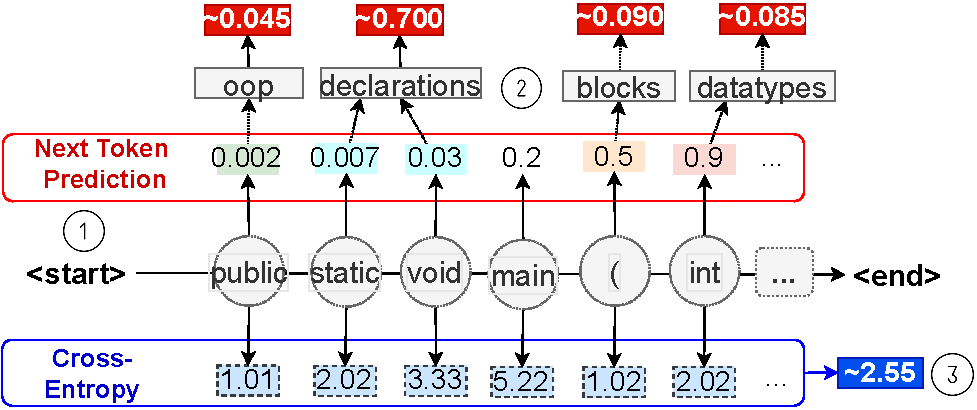
\includegraphics[width=0.9\textwidth]{graphics/preliminaries/fig_2_performance.pdf}
		%\vspace{-0.3cm}
		\caption{Potential Outcomes are Prediction Performance of  \nlms: Cross-Entropy $(Y_g)$ and Next Token Predictions $(Y_l)$.}
        %\vspace{-0.1cm}
        \label{fig:performance}
\end{figure}

A major conjecture in interpretability research is that \nlms are more understandable when they \textit{reflect human knowledge} \citep{Kim2018InterpretabilityTCAV}. One way of determining whether a model reflects human knowledge is testing it to see whether or not it operates (or predicts) \textit{similar to how a human would operate}. \codegen accomplishes this by mapping the complex interactions present in both Global $Y_g$ and Local $Y_l$ Potential Outcomes of a \nlm to human interpretable PL features and testbeds. Below we provide a motivating example for this mapping function, which we formally introduce in Definition \ref{def:taxonomy}:

\begin{exmp}
\label{exmp:outcome}
Consider the situation where a developer inserts a \texttt{\small `('} character after the \texttt{\small `main'} keyword in a function declaration in Java ({\circled{1}}-Fig.~\ref{fig:performance}). Inherently, a developer mentally rationalizes several things such as the concept of a function declaration and expected Java syntax. If a \nlm is able to make a similar prediction, it suggests to us that it has \textit{statistically learned} some understanding of the concept of a function declaration and corresponding syntax. Thus, we assert that by ascribing human-interpretable properties, and in particular code-related properties, to model predictions, and then analyzing the statistical properties of those predictions, we can begin to learn how well a given \nlm reflects human knowledge. We propose a \textit{Structural Code Taxonomy} $\mathcal{H}$ to bridge this interpretability gap.
\end{exmp}

\marginnote{
    \begin{definition}
    \label{def:taxonomy}
    \textbf{Structural Code Taxonomy.} In programming languages (PL), different types of tokens retain different semantic meanings. For instance \texttt{\small `='} and \texttt{\small `<'} are common \operators. As such, we can group tokens into semantically meaningful \textit{categories}. Fig.~\ref{fig:taxonomy} depicts an initial version of \codegen's taxonomy derived from Java. These features will allow \codegen to assign semantic meaning to predicted tokens $\hat{w_t}$. The taxonomy comprises high-level properties of code using a \textbf{mapping function} $\phi_{\mathcal{H}}: \vec{w} \to \vec{h} $, where the vector $\vec{w}$ corresponds to tokens of the vocabulary $\mathcal{V}$. Each token in a sequence $w$ is assigned to a taxonomy category $h \in \mathcal{H}$.
    \end{definition}
}

With our categories $\mathcal{H}$, researchers and practitioners can easily associate \nlm performance (\ie $Y_g$ or $Y_l$) to particular structural code attributes. As such, by using our structural code taxonomy, \codegen allows for \nlm predictions to be interpreted in a developer-centric way. These categories represent a “base” case as the keywords of any PL can likely be grouped into interpretable categories. This is why anyone using \codegen can \textit{easily define their own mapping function} $\phi_{\mathcal{H}}$ (\eg using coupling and cohesion metrics), and stipulate them in a JSON-like configuration file. For instance, a researcher working to analyze how well \nlms learn to predict cryptographic APIs could define a taxonomy based upon “safe” and “unsafe” APIs.

 \begin{marginfigure}
		\centering
		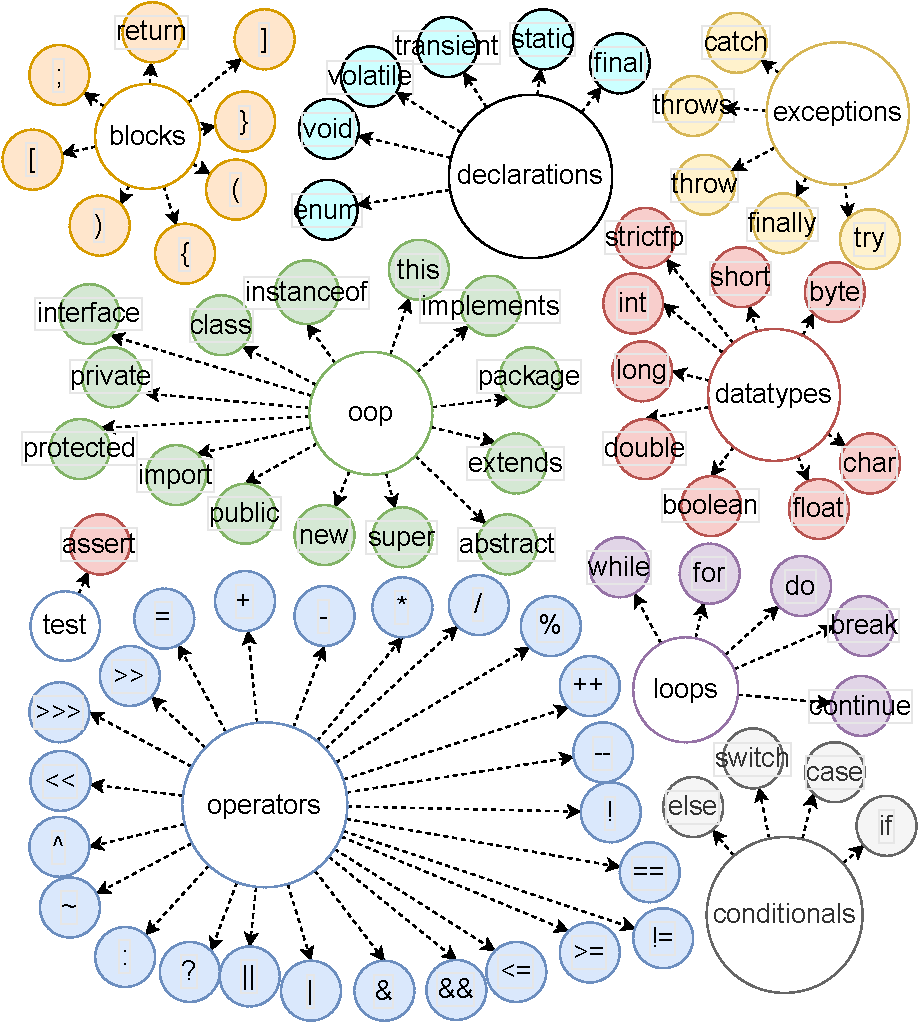
\includegraphics[width=\textwidth]{graphics/preliminaries/fig_3_taxonomy.pdf}
		\caption{Structural Code Taxonomy $\mathcal{H}$ for Java}
        \label{fig:taxonomy}
\end{marginfigure}

\subsection{Stage 2 (St$_2$): Computing Causal Inference (CI)}
%Definition of Causal Inference
According to Pearl \& Mackenzie \citep{Pearl2018Causality}, CI seeks answers to questions of association (\textit{what is?}), counterfactual interventions (\textit{what if?}), and pure counterfactuals (\textit{why?}). The authors introduce the concept of \textit{levels of causation} to match distinct levels of cognitive ability with concrete actions: seeing~(\textit{level 1}), doing~(\textit{level 2}), and imagining~(\textit{level 3}). Our proposed analysis is primarily concerned with levels 1 \& 2. Level 1 causation, namely association, $p(Y|T)$ is estimated by using typical correlation methods (\eg Pearson, Spearman, or Covariance) in addition to functional associations such as $y=g(t)$, which can be predicted with regressions or ML methods. For binary treatments similar to the ones we used in $T_{[data]}$ (\eg Buggy/Fixed, Commented/Uncommented, Clone1/Clone2), we opt to employ Pearson correlations and Jensen-Shannon distance as association estimand for level 1 causation. We will now formally define each of these below \david{Contextualize the functions below}.

\marginnote{
\begin{definition}
\label{def:js}
\textbf{Jensen-Shannon Distance (JS).} The Jensen-Shannon divergence (JSD) overcomes the asymmetric computation of the KL divergence and provides a measure of difference between distributions Eq.~\ref{eq:js_divergence}. The JS distance is the square of the JS divergence $p(Y|T)\approx JS(Y^{T=0},Y^{T=1}) = JSD(Y^{0},Y^{1})^2$. JS is proportional to the influence of $T$ on $Y$, which measure the separation of the distributions $Y^{0},Y^{1}$. The notation $Y^{T=0}$ refers to the potential outcomes observed under the treatment $T=0$. 

\end{definition}
}

\begin{subequations}
    {%\tiny %footnotesize
    \begin{align}
     JSD(Y^{0}=y^0,Y^{1}=y^1) &&= \label{eq:js_divergence-1}\\
     \frac{1}{2}\left[ D_{KL}\left(y^0||\frac{y^0+y^1}{2}\right) + D_{KL}\left(y^1||\frac{y^0+y^1}{2}\right)\right] &&= \label{eq:js_divergence-2}
    \end{align}
    }
\label{eq:js_divergence}
\end{subequations} 

\begin{exmp}
\label{exmp:js}Imagine we wish to understand the correlation between syntactic changes, \ie variable renaming, alterations in white space, \etc and a \nlms performance. One way we can study this is through computing the association of Cross-Entropy values $Y$ under two treatments, the first $T=0$, would be an unaltered code snippet and the second $T=1$ would be its Type III clone. Computing this association can be done using the JS distance $p(Y|T)\approx JS(Y^0,Y^1)$ as defined in Def.~\ref{def:js} for four models. Fig.~\ref{fig:jssimilarity} shows the distributions of $Y^0$ and $Y^1$ with their distances after applying bootstrapping as an example.

\begin{figure}[th]
  \centering
  \begin{subfigure}[b]{0.46\linewidth}
    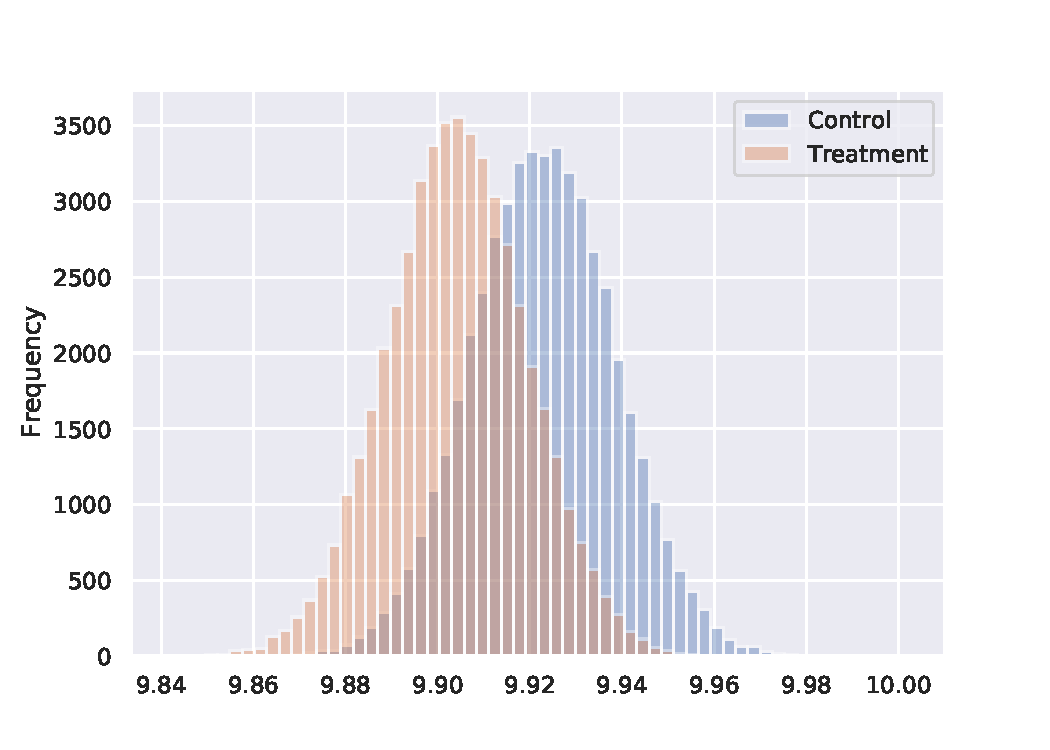
\includegraphics[width=\linewidth]{graphics/preliminaries/association/cross-entropy-rnn1-distribution-clone3-300dpi.pdf}
    %  \caption{RNN1.}
  \end{subfigure}
  \begin{subfigure}[b]{0.46\linewidth}
    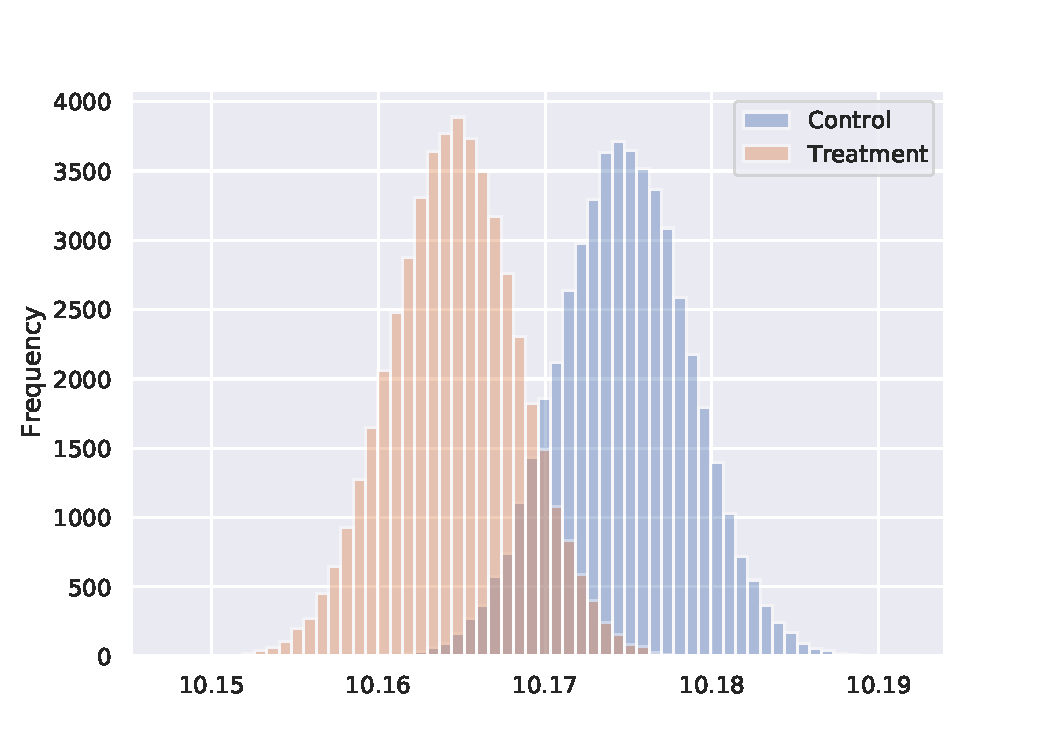
\includegraphics[width=\linewidth]{graphics/preliminaries/association/cross-entropy-gru1-distribution-clone3-300dpi.pdf}
    % \caption{GRU1.}
    % \vspace{0.2cm}
  \end{subfigure}
  \begin{subfigure}[b]{0.46\linewidth}
    % \vspace{-0.2cm}
    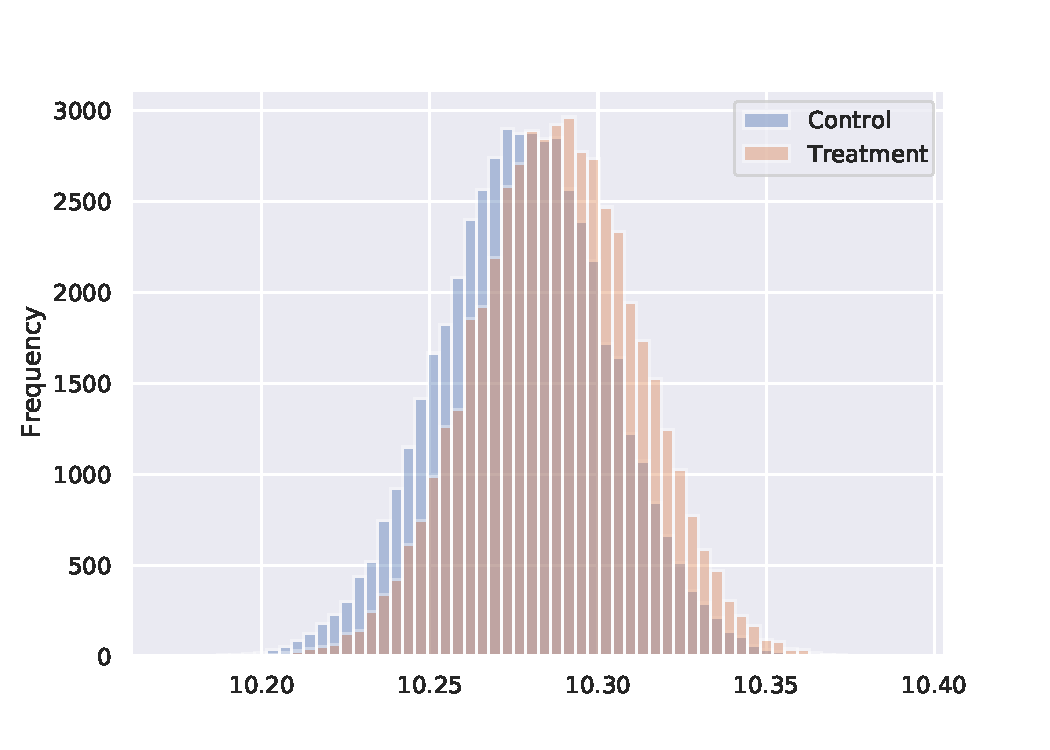
\includegraphics[width=\linewidth]{graphics/preliminaries/association/cross-entropy-tf1-distribution-clone3-300dpi.pdf}
    % \caption{TF1.}
  \end{subfigure}
  \begin{subfigure}[b]{0.46\linewidth}
    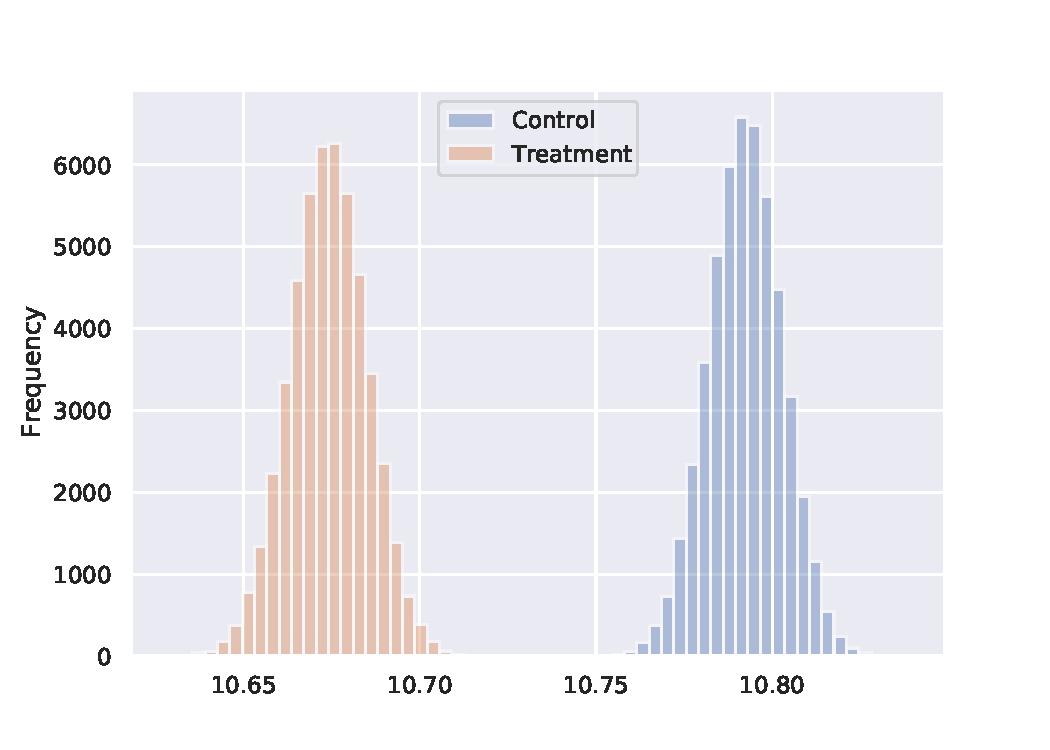
\includegraphics[width=\linewidth]{graphics/preliminaries/association/cross-entropy-tf2-distribution-clone3-300dpi.pdf}
    % \caption{TF2.}
  \end{subfigure}
  \vspace{-0.2cm}
  \caption{\datainterII Intervention (\BigCloneIIITB) for Global Performance: Bootstrapped Cross-Entropy. Top Left: \rnn ($JS=0.3$), Top Right: \gru ($JS=0.8$), Bot Left: \tf ($JS=0.6$), Bot Right: \tfi ($JS=1$).}
  \label{fig:jssimilarity}
  \vspace{-0.3cm}
\end{figure}

\end{exmp}

Now, if we want to go beyond \textit{``what is''} type questions, we must move past simple correlations and association. This requires the $do-operator$ found in level 2, causation $p(y|do(t))$. Specifically, it is estimated for a population (\ie SE dataset) by computing an \textit{Average Treatment Effect} based on the Def.~\ref{def:effect} introduced in Sec.~\ref{sec:pre-ci4se}.

\marginnote{
\begin{definition}
\label{def:ate}
\textbf{Average Treatment Effect (ATE)} Defining the first intervention as $do(T=1)$ and the second by $do(T=0)$, the Average Treatment Effect is the population average of the difference of causal effects of each code snippet $x$.  
\end{definition}
}

\david{Contextualize the functions below}
\begin{subequations}
    \begin{align}
     ATE = \mathbb{E}_{x\sim p(x)}[Y=y|x,do(T=t)]  &= \label{eq:ate-1}\\
     \mathbb{E}_{x\sim p(x)}[ \mathbb{E}[Y|x,do(T=1)] - \mathbb{E}[Y|x,do(T=0)] ] &= \label{eq:ate-2}\\
     \mathbb{E}_{x\sim p(x)}[ \mathbb{E}[Y^{1}|x,T=1] - \mathbb{E}[Y^{0}|x,T=0] ] &= \label{eq:ate-3}
    \end{align}
\label{eq:ate}
\end{subequations} 


ATE can be computed in two steps as follows:

\textbf{a. Identifying Causal Effects.} Once the SCM (similar to Fig.~\ref{fig:scm}) is constructed, \codegen applies various techniques (\ie backdoor-criterion and instrumental variables) to determine the adjustment formula Eq.~\ref{eq:effect}, which will control for confounding common causes when computed. For our case study, the causal effect $p(Y|do(T))$ is computed, which will be done in the next step, based on the following causal graph: data-based $T_{[data]}$ and parameter-based $T_{[hyp]}$ treatments; SE covariates $Z \in SE_{metrics}$; and potential outcomes $Y_l, Y_g$.

\textbf{b. Estimating Causal Effects.} Next, \codegen estimates the causal effect using statistical and ML methods based on the adjustment formula from the previous step. \codegen computes \textit{Propensity Score Matching} for binary SE treatments (\ie Buggy/Fixed) and \textit{Linear Regressions} for SE discrete treatments (\eg layers, units, or heads). We refer interested readers to the \textit{doWhy} documentation for the full process details \citep{dowhy}. For completeness, we will now show how to estimate a causal effect assuming a binary treatment as an example. Eq.~\ref{eq:ate} shows the formal definition of an \textit{ATE}. We can derive the final expression by applying the law of total expectations and the ignorability assumption  $Y \perp\!\!\!\perp  Z|T$, where the potential outcomes $Y$ are independent of treatment assignments conditioned on covariates $Z$ \citep{Pearl2009Causality}. That is, the effects of the hidden common causes $Z$ and missing data are ignored. In Eq.~\ref{eq:ate}, the term $\mathbb{E}[Y^1|x,T=1]$ represents the expected value of a potential outcome under an observable treatment (\ie FixedCode). Similarly, the term $\mathbb{E}[Y^0|x,T=0]$ represents an expected value of a potential outcome under an observable control (\ie BuggyCode). Both terms are quantities that can be \textit{estimated from data}. Covariate adjustment (in Eq.~\ref{eqn:do-all-lines}), propensity score (in Eq.~\ref{eq:effect-3}), and linear regression are some of the estimation methods that we employ to estimate the $ATE$. Their usage depends upon the type of the treatment variable (\ie binary, discrete, or continuous) and causal graph assumptions.

\subsection{Stage 3 (St$_3$): Evaluating Causal Effects}
The previous causal estimation can be validated using \textit{refutation methods} that calculate the robustness of the causal estimate. In essence, the refutation methods apply random perturbations to the original causal graph to test for robustness of the estimated $ATE$. We chose four methods for our analysis: Adding a random common cause or covariate $\mathcal{R}_1$, adding an \textit{unobserved} common cause or covariate $\mathcal{R}_2$, replacing the treatment with a random variable or placebo $\mathcal{R}_3$, and removing a random subset of the data $\mathcal{R}_4$. For robustness, we expected that $\mathcal{R}_1$, $\mathcal{R}_2$, and $\mathcal{R}_4$ values were close to the $ATE$ (Eq.~\ref{eq:ate}). Conversely, the placebo $\mathcal{R}_3$ should tend to zero.

In addition to measuring refutation methods, it is relevant to identify cases of \textit{spurious correlations} (\ie \textit{Confounding Bias}) or cases where $p(Y|T)\neq p(Y|do(T))$. Typically, association is not causation due to the influence of a common cause or confounding variable $Z$. Such a variable is the one that is being controlled for or adjusted by means of Eq.~\ref{eqn:do-all-lines}. Nonetheless, we can still compute the correlation $d(Y|Z)$ to assess the variables that are actually affecting potential outcomes. 

 \begin{marginfigure}
		\centering
		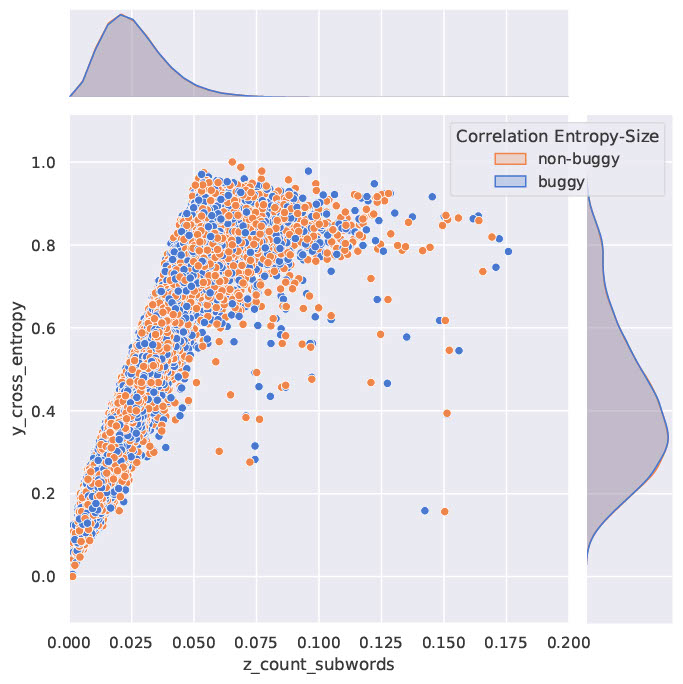
\includegraphics[width=\textwidth]{graphics/fig_4_covariates_corr.jpg}
		\caption{ \textit{Spurious Correlation} between the \textit{Number of Subwords} common cause and Cross-Entropy values ($p(Y|Z)\approx0.87$) for the \datainterI intervention generated from \tf. } 
        %\vspace{-0.5cm}
        \label{fig:covariate}
\end{marginfigure}

\begin{exmp}
\label{exmp:confounding}

Consider the \datainterI intervention where $T$ is Buggy/Fixed code, $Y$ is the cross-entropy of each of method of the dataset \BuggyTB, and $Z$ is the \textit{Number of Subwords} for each method. There exists a spurious correlation after calculating JS and ATE, $p(Y|T)\approx0.67$ and $p(Y|do(T))\approx-0.0002$. One possible explanation is that the common cause $Z$ is confounding the relationship between the treatment and the outcome. Fig.~\ref{fig:covariate} depicts the influence of $Z$ on the potential outcome $Y$ for BuggyCode ($p(Y|Z,T=Buggy)\approx0.87$) and FixedCode ($p(Y|Z,T=Fixed)\approx0.86$). Blue and orange points in the plot are code snippets from the dataset. These points are equally distributed, which suggest that the \datainterI intervention has a negligible impact on the Cross Entropy. 
\end{exmp}

%------------------------------------------------

\section{Case Study Design in Code Generation}
\label{sec:design-conditioned}

%Intro
In order to illustrate the insights that \codegen can enable, we present a case study that serves as a practical application of our interpretability method by analyzing two popular \nlms: RNNs and Transformers. In this section, we detail the methodological steps we took to configure our models and process our datasets. In addition, we designed our methodology for causal understanding following Pearl~\etal's guidelines \citep{Pearl2016Causality,Sharma2021DoWhyAssumptions}. We adopted these guidelines to formulate two research questions: \ref{rq:causal} SE Intervention Effects and \ref{rq:eval} Stability Causation.

\begin{enumerate}[label=\textbf{RQ$_{\arabic*}$:}, ref=\textbf{RQ$_{\arabic*}$}, wide, labelindent=5pt]\setlength{\itemsep}{0.2em}
      \item \label{rq:causal} {\textit{To what extent do SE data and model interventions affect code prediction performance?}} 
       \begin{enumerate}[label=\textbf{RQ$_{1.\arabic*}$:}, ref=\textbf{RQ$_{1.\arabic*}$}, wide, leftmargin=0.5cm]\setlength{\itemsep}{0.2em}
        \item \label{rq:global}{\textit{What is the influence of our interventions on global performance?}}
        \item \label{rq:local}{\textit{What is the influence of our interventions on local performance?}}
        \end{enumerate}
      \item \label{rq:eval} {\textit{How robust are the treatment effects based on SE interventions?}}
\end{enumerate}

\begin{table*}[b]
\centering
\caption{Counterfactual Interventions Case Study. NLMs include Recurrent Nets (GRUs) and Transformers (TFs). 
%The units of TFs are heads [hds]. 
}
\vspace{0.2cm}
\label{tab:method}

%\scalebox{0.65}{%
\resizebox{\textwidth}{!}{
%%%%%%%%%%%%%%%%%

\begin{tabular}{@{}llllll|llll@{}}
\toprule
\multicolumn{6}{c|}{\textbf{Case Study Methodology}} &
  \multicolumn{4}{c}{\textbf{\nlms Training}} \\ \midrule
\multicolumn{4}{c}{\textit{\textbf{\begin{tabular}[c]{@{}c@{}}Counterfactual\\ Interventions\end{tabular}}}} &
  \multicolumn{2}{c|}{\textit{\textbf{\begin{tabular}[c]{@{}c@{}}Proposed Experiments\\ Global and Local\end{tabular}}}} &
  \multicolumn{1}{c}{\textit{\textbf{RNNs}}} &
  \multicolumn{1}{c|}{\textit{\textbf{Transformers}}} &
  \multicolumn{1}{c}{\textit{\textbf{Hyper.}}} &
  \multicolumn{1}{c}{\textit{\textbf{Val.}}} \\ \midrule
\multicolumn{1}{c}{\textit{Type}} &
  \multicolumn{1}{c}{\textit{Interv.}} &
  \multicolumn{1}{c}{\textit{Case}} &
  \multicolumn{1}{c}{\textit{Associated Dataset}} &
  \multicolumn{1}{c}{\textit{Avg. Causation}} &
  \multicolumn{1}{c|}{\textit{Correlation}} &
  \textit{\nlm $_{lyr,unt}$} &
  \multicolumn{1}{l|}{\textit{\nlm$_{lyr,hds}$}} &
  \multirow{6}{*}{\begin{tabular}[c]{@{}l@{}}dropout RNN\citep{Karampatsis2020BigCode}\\ dropout TF\\ optimizer\citep{Kingma2015AdamAM}\\ learning rate\\ beta1$|$beta2\\ epsilon\\ epochs\\ batch RNN$|$TG\end{tabular}} &
  \multirow{6}{*}{\begin{tabular}[c]{@{}l@{}}0.5\\ 0.l\\ adam\\ 1e-3\\ 0.9\\ 1e-7\\ 64\\ 512$|$128\end{tabular}} \\ \cmidrule(r){1-8}
\multirow{3}{*}{\textit{Data}} &
  $T_{dat0}$ &
  \datainterI &
  \BuggyTB\citep{Tufano2019LearningBug-Fixes} &
  \colorbox{blue!10}{$p(Y_{g,l}|do(T_{dat0}))$} &
  \colorbox{blue!10}{$p(Y_{g,l}|T_{dat0})$} &
  \multirow{5}{*}{\begin{tabular}[c]{@{}l@{}}\rnn\\ \gru\\ \grui\\ \gruii\\ \gruiii\\ \gruiv\end{tabular}} &
  \multicolumn{1}{l|}{\multirow{5}{*}{\begin{tabular}[c]{@{}l@{}}\tf\\ \tfi\\ \tfii\end{tabular}}} &
   &
   \\
 &
  $T_{dat1}$ &
  \datainterIII &
  \CommentsTB\citep{husain2019codesearchnet} &
  \colorbox{blue!10}{$p(Y_{g,l}|do(T_{dat1}))$} &
  \colorbox{blue!10}{$p(Y_{g,l}|T_{dat1})$} &
   &
  \multicolumn{1}{l|}{} &
   &
   \\
 &
  $T_{dat2}$ &
  \datainterII &
  \begin{tabular}[c]{@{}l@{}}\BigCloneIITB\citep{Svajlenko2015EvaluatingBigCloneBench}\\ \BigCloneIIITB\citep{Svajlenko2015EvaluatingBigCloneBench}\end{tabular} &
  \colorbox{blue!10}{$p(Y_{g,l}|do(T_{dat2}))$} &
  \colorbox{blue!10}{$p(Y_{g,l}|T_{dat2})$} &
   &
  \multicolumn{1}{l|}{} &
   &
   \\ \cmidrule(r){1-6}
\multirow{2}{*}{\textit{Model}} &
  $T_{hyp0}$ &
  \modelinterI &
  \multirow{2}{*}{\training\citep{husain2019codesearchnet}} &
  \colorbox{blue!10}{$p(Y_{g,l}|do(T_{hyp0}))$} &
  \colorbox{blue!10}{$p(Y_{g,l}|T_{hyp0})$} &
   &
  \multicolumn{1}{l|}{} &
   &
   \\
 &
  $T_{hyp1}$ &
  \modelinterII &
   &
  \colorbox{blue!10}{$p(Y_{g,l}|do(T_{hyp1}))$} &
  \colorbox{blue!10}{$p(Y_{g,l}|T_{hyp1})$} &
   &
  \multicolumn{1}{l|}{} &
   &
   \\ \bottomrule
\end{tabular}


%%%%%%%%%%%%%%%%%%


}
\vspace{-0.35cm}

\end{table*} 

\codegen adapts causal inference theory to aid in providing explanations for both global $Y_g$ (\ref{rq:global}) and local $Y_l$ (\ref{rq:local}) prediction performance of given \nlms. Before \codegen can be performed, a researcher or practitioner making use of our method must select the \nlms and define \textit{hyper-parameter variations} $T_{[hyp]}$ and \textit{data perturbations} $T_{[data]}$ that they would like to examine in Stage 1 ($St_1$). Here, \textit{hyper-parameter variations} are essentially different configurations of a given model according to attributes such as capacity (layers) or the types of layers. Additionally, the researcher must define their code \textit{testbeds}. \codegen offers the possibility of adding additional testbeds with data \textit{perturbations} that represent a set of SE-based interventions or Application Settings. After defining and estimating the causal effect (\ref{rq:causal}) of proposed interventions in Stage 2 ($St_2$), \codegen helps to evaluate the robustness of ATE's results by performing refutation methods proposed in Stage 3 ($St_3$) (\ref{rq:eval}).

\subsection{Context: Data Processing \& Model Training}
To train our \nlms we made use of the Java portion of the commonly used \training Challenge dataset~\citep{husain2019codesearchnet}, which consists of a diverse set of methods (mts) from GitHub \citep{github}. \training is split into a training, validation, and test set. For the testbeds for interpreting the performance of our \nlms using \codegen, we collected four datasets from the \textit{CodeXGLUE} project that contain control and treatment groups \citep{DBLP:journals/corr/abs-2102-04664}. Tab.~\ref{tab:method} shows the generated testbeds containing parallel corpora for understanding the impact of buggy code (\BuggyTB: 64,722 mts), the impact of code documentation (\CommentsTB: 6,664 mts), and syntactic alterations on semantically equivalent snippets based on type II (\BigCloneIITB: 666 mts) and type III (\BigCloneIIITB: 8,097 mts) clones from \BigCloneTB. The only additional filtering we performed on the training, validation, and testbeds was the removal of methods that contain any non-ASCII characters and, for the \CommentsTB, removal of methods that do not have comments.  We derived the uncommented portion of the \CommentsTB by removing any existing comments from the Java test set of the \training dataset.

We performed Byte Pair Encoding (BPE) tokenization \citep{sennrich2015neural} across all testbeds before they were processed by our studied \nlms. BPE has shown to be extremely beneficial for training \nlms on code to overcome the \textit{out-of-vocabulary} problem \citep{Karampatsis2020BigCode}. We trained a BPE tokenizer on 10\% of our training data and used a vocabulary size of 10K. Due to the tokenization process of BPE, some subtokens contained multiple reserved keywords or characters if they appeared frequently together. This was problematic for our interpretability analysis since the function $\phi_{\mathcal{H}}$ relies on the ability to map model predictions to our structural taxonomy. Having certain reserved keywords and tokens merged into BPE subtokens would make it impossible for us to perform this mapping. Therefore, we fixed all reserved keywords and tokens (Fig.~\ref{fig:taxonomy}) to be detected by our trained BPE model.

As for the model training, we used Tensorflow and Pytorch \citep{tensorflow2015-whitepaper, pytorch} (Huggingface's Transformers library \citep{wolf2020transformers}) for creating and training our different models. Our $RNN$ and $TF$ models were trained on \training Java training set. All models reached optimal capacity as they all early terminated to prevent overfitting, with a patience of $5$ epochs without improvement on cross-entropy of at least $1\text{e-2}$. Additionally, we added a \textit{start of sentence} token to the beginning of the input, padded and truncated all inputs to $300$. The training was executed on a 20.04 Ubuntu with an AMD EPYC 7532 32-Core CPU, A100 NVIDA GPU with 40GB VRAM, and 1TB RAM.

\subsection{Case Study Methodology}
We provide an overview of our case study summarized in Tab.~\ref{tab:method}, which follows the \codegen methodology introduced in Sec.~\ref{sec:appII-approach}. This section provides the details regarding how we instantiated \codegen's methodology for our studied models and testbeds. On one hand, we empirically estimated $p(Y|T)$ using two methods: Pearson correlations and Jensen-Shannon Similarities (explained in Def.~\ref{def:js}). On the other hand, we estimated $p(Y|do(T))$ using the \textit{doWhy} library \citep{Sharma2021DoWhyAssumptions} and ATE (explained in Def.~\ref{def:ate}).

\codegen is extensible and researchers can define their own treatments. In our case study, we suggested three \textit{data interventions} $T_{[data]}$ (see row \textit{Data} in Tab.~\ref{tab:method}). In addition, the aim of the syntax analysis was to determine how robust \nlms are in the presence of minor and major syntactic variations of semantically equivalent code snippets. That is, we assessed how semantic preserving changes affect code generation. Since there is no natural split for the different clone types, we were unable to perform a causal analysis on the \BigCloneTB dataset using the typical control and treatment settings. This is because the choice of one clone compared to another is arbitrary when evaluating the set of what \BigCloneTB calls \textit{function$_1$} and \textit{function$_2$} methods. Therefore, instead of our standard covariates, we used the differences between \textit{function$_1$} and \textit{function$_2$} of the different clone types. Specifically, we used the Levenshtein Distance $T_{[dat1]}$, a measure of the difference between two sequences in terms of the necessary edit operations (insert, modify, and remove) needed to convert one sequence into the other, to approximate a treatment where one method was \textit{refactored} into another method by a specific number of edit operations. This formulation allowed us to avoid needing a natural split between \textit{function$_1$} and \textit{function$_2$} and focused on how syntactic differences of methods that perform the same function, \ie semantically similar, affects our models. 

As for the \textit{model interventions} $T_{[hyp]}$ (see row \textit{Model} in Tab.~\ref{tab:method}), our case study consists of an investigation of two different \nlm architectures. We also investigated how layer and unit variations in each architecture affect their performance. We made use of two different types of RNN architectures, a ``base'' model and a model that includes Gated Recurrent Units (GRU). Additionally, we studied a GPT-based Transformer model~\citep{Cho2014GRU, Radford2018ImprovingLU} for our autoregressive model. We chose these two models because RNNs have been extremely popular in SE \citep{watson2020dl4se} and Transformers have recently gained popularity due to the high performance they have achieved in the NLP domain~\citep{Mastropaolo2021StudyingTasks}.

%------------------------------------------------

\section{Results and Discussion}
\label{sec:results}

\subsection{\ref{rq:global} SE Intervention on Global Performance}

% Please add the following required packages to your document preamble:
% \usepackage{multirow}
\begin{table*}[b]
\centering
\caption{Causal Interventions $p(Y_g|do(T))$ and Associations $p(Y_g|T)$ of Global Performance across models and datasets.}
\vspace{0.2cm}
\label{tab:results_global}

%\scalebox{0.55}{%<-------SCALLING
\resizebox{\textwidth}{!}{

\begin{tabular}{l|rrr|rrr|rrrrrl|rr}
\hline
\multirow{2}{*}{\textbf{\begin{tabular}[c]{@{}l@{}}Counterfactual  \\ Interventions $T$ \end{tabular}}} & \multicolumn{3}{c|}{\multirow{2}{*}{\textbf{\begin{tabular}[c]{@{}c@{}}\datainterI (BuggyTB)\\ $T_{dat0}$\end{tabular}}}} & \multicolumn{3}{c|}{\multirow{2}{*}{\textbf{\begin{tabular}[c]{@{}c@{}}\datainterIII (CommentsTB)\\ $T_{dat1}$\end{tabular}}}} & \multicolumn{6}{c|}{\textbf{\begin{tabular}[c]{@{}c@{}}\datainterII (BigClone2/3TB)\\ $T_{dat2}$\end{tabular}}}                                                                                                       & \multicolumn{2}{c}{\multirow{2}{*}{\textbf{\begin{tabular}[c]{@{}c@{}}\modelinterI (CodeSearchNet)\\ $T_{hyp0}$\end{tabular}}}} \\ \cline{8-13}
                                                                                                          & \multicolumn{3}{c|}{}                                                                                                     & \multicolumn{3}{c|}{}                                                                                                          & \multicolumn{3}{c|}{\textbf{BigClone2TB}}                                                                 & \multicolumn{3}{c|}{\textbf{BigClone3TB}}                                                                 & \multicolumn{2}{c}{}                                                                                                            \\ \hline
\nlm                                                                                                      & \multicolumn{1}{c}{\textit{\rnn}}       & \multicolumn{1}{c}{\textit{\gru}}      & \multicolumn{1}{c|}{\textit{\tf}}      & \multicolumn{1}{c}{\textit{\rnn}}        & \multicolumn{1}{c}{\textit{\gru}}        & \multicolumn{1}{c|}{\textit{\tf}}        & \multicolumn{1}{c}{\textit{\rnn}} & \multicolumn{1}{c}{\textit{\gru}} & \multicolumn{1}{c|}{\textit{\tf}} & \multicolumn{1}{c}{\textit{\rnn}} & \multicolumn{1}{c}{\textit{\gru}} & \multicolumn{1}{c|}{\textit{\tf}} & \multicolumn{1}{c}{\textit{\gru}}                               & \multicolumn{1}{c}{\textit{\tf}}                              \\ \hline
\textit{Association}                                                                     & \colorbox{blue!10}{0.730$_{JS}$}                            & 0.230$_{JS}$                           & \colorbox{blue!10}{0.670$_{JS}$}                           & \textbf{0.180$_{JS}$}                    & 0.220$_{JS}$                             & 0.250$_{JS}$                             & 0.45$_{PR}$                       & 0.598$_{PR}$                      & \multicolumn{1}{r|}{0.452$_{PR}$} & -0.056$_{PR}$                     & 0.14$_{PR}$                       & -0.14$_{PR}$                      & -0.093$_{PR}$                                                   & -0.485$_{PR}$                                                 \\
\textit{Causal Eff. ATE}                                                                                  & -0.0003                                 & -2.33E-05                              & -0.0002                                & 0.0023                                   & 2.90E-05                                 & 0.0026                                   & 0.6288                            & \colorbox{blue!10}{\textbf{0.8713}}                   & \multicolumn{1}{r|}{0.5635}       & -0.1042                           & 0.1085                            & -0.2739                           & -0.0058                                                         & -0.0124                                                       \\
\textit{Random Cause $\mathcal{R}_1$}                                                                               & -0.0003                                 & -2.45E-05                              & -0.0002                                & 0.0011                                   & -0.0004                                  & 0.0015                                   & 0.6297                            & 0.8720                            & \multicolumn{1}{r|}{0.5651}       & -0.1043                           & 0.1084                            & -0.2741                           & -0.0058                                                         & -0.0124                                                       \\
\textit{Unobserved Cause $\mathcal{R}_2$}                                                                           & -0.0003                                 & 1.54E-05                               & -0.0001                                & 0.0002                                   & -0.0001                                  & 0.0007                                   & 0.2950                            & 0.4257                            & \multicolumn{1}{r|}{0.2737}       & -0.0800                           & 0.0830                            & -0.2168                           & -0.0050                                                         & -0.0108                                                       \\
\textit{Placebo $\mathcal{R}_3$}                                                                                          & 0.0001                                  & 1.44E-05                               & 0.0001                                 & 0.0006                                   & -1.33E-05                                & 0.0006                                   & -                               & -                               & \multicolumn{1}{r|}{-}          & -                               & -                               & \multicolumn{1}{r|}{-}          & -0.0001                                                         & -2.77E-05                                                     \\
\textit{Remove Subset $\mathcal{R}_4$}                                                                                    & -0.0003                                 & -3.68E-05                              & -0.0002                                & 0.0012                                   & -0.0003                                  & 0.0016                                   & -                               & -                               & \multicolumn{1}{r|}{-}          & -                               & -                               & \multicolumn{1}{r|}{-}          & -0.0058                                                         & -0.0124                                                       \\ \hline
\end{tabular}
}
\end{table*}

Tab. \ref{tab:results_global} gives an overview of the different associative and interventional effects across our different models and datasets in terms of global performance. Note that the correlation row includes both Pearson and Jensen-Shannon distances. For the \datainterII intervention, the association values in Tab.~\ref{tab:results_global} indicate that Levenshtein ``edit'' distance between Type II clone pairs has a tendency to be positively correlated with cross-entropy values $p(Y_g|T_{dat2})\approx0.60$ for \gru. By contrast, for the Type III clones, no strong correlations were detected between syntactic and global performance differences for any of our \nlms. Nonetheless, we discovered an appreciably strong causal effect between the Levenshtein distance of clone pairs and the difference in cross-entropy with a maximum of $p(Y_g|do(T_{dat2}))=0.87$ for \gru on Type II. This suggests that our models are causally influenced by slight and major changes in syntax of programs such as white space and variable names. This is not a desired effect for code \nlms as developers have their own coding style and conventions, a \nlm should perform similarly independent from the syntactic alterations. 

For \datainterI intervention, it is apparent that both \rnn and \tf exhibit considerably high JS distances. However, after controlling for SE covariates, we found that such correlations were spurious since ATEs are relatively small for the three models. The confounding is explained in Fig.~\ref{fig:covariate}, where the number of subwords per method is affecting the cross entropy directly beyond the \datainterI intervention. We have identified more confounding variables for our proposed interventions such as \textit{the Number of Unique Words}, \textit{MaxNextedBlocks}, and \textit{Cyclomatic Complexity}. However, the variable that most influence prediction performance is the \textit{Number of Subwords} per method. Similar results were found for \datainterIII (TypeIII) interventions after adjustment of covariates. We saw a tendency to null causal effects, meaning, for example, that there is little to no causal influence of removing comments from the code or applying Type III syntactic changes on snippets.

As for model-based interventions, \modelinterI and \modelinterII interventions have a tendency to be negatively correlated to and to causally influence the cross-entropy. For instance, the number of units negatively affect global performance by $p(Y_g|T_{hpy1})\approx-0.084$ for \gru, which is a result align with expected DL experimentation on hyperparameters. Smaller values of cross-entropy are observed once the number of layers and units increases.

\marginnote{
\textit{\ref{rq:global} Global Causal Findings:} 
In contrast to our correlation analysis, after controlling for covariates, we found that \datainterI, \datainterIII, and \datainterII (Type III) had a very small causal effect on cross-entropy across our models. We observed a consistent causal effect on the performance in the presence of syntactic changes (Type II and III) present in our code clone testbeds. Only Transformers had an appreciable correlation and causation between increasing the number of layers and the overall performance in terms of cross-entropy.
}

\subsection{\ref{rq:local} SE Intervention on Local Performance}
\begin{table*}[b]
\centering
\caption{Local Association Results $p(Y_l|T)$ are \textit{Jensen-Shannon Dist}. Causal Effects are ATEs $p(Y_l|do(T))$ \\(bold:strong corr., background:best effect)}
\vspace{0.2cm}
\label{tab:resultsLocalJS}

\scalebox{0.60}{%


%%%%%%%%%%%%%%%%%

\begin{tabular}{@{}l|rrrrrr|rrrrrr@{}}
\toprule
\textbf{\begin{tabular}[c]{@{}l@{}}Counterfactual  \\ Interventions $T_{data}$\end{tabular}} &
  \multicolumn{6}{c|}{\textbf{\begin{tabular}[c]{@{}c@{}}\datainterI \\ $T_{dat0}$\end{tabular}}} &
  \multicolumn{6}{c}{\textbf{\begin{tabular}[c]{@{}c@{}}\datainterIII\\ $T_{dat1}$\end{tabular}}} \\ \midrule
\nlm &
  \multicolumn{3}{c}{\textit{\gru}} &
  \multicolumn{3}{c|}{\textit{\tf}} &
  \multicolumn{3}{c}{\textit{\gru}} &
  \multicolumn{3}{c}{\textit{\tf}} \\ \midrule
\textbf{Categories} &
  \multicolumn{1}{c}{\textit{\begin{tabular}[c]{@{}c@{}}Association\\ \assoJS\end{tabular}}} &
  \multicolumn{1}{c}{\textit{\begin{tabular}[c]{@{}c@{}}Causal Eff.\\ ATE\end{tabular}}} &
  \multicolumn{1}{c}{\textit{\rfi}} &
  \multicolumn{1}{c}{\textit{\begin{tabular}[c]{@{}c@{}}Association\\ \assoJS\end{tabular}}} &
  \multicolumn{1}{c}{\textit{\begin{tabular}[c]{@{}c@{}}Causal Eff.\\ ATE\end{tabular}}} &
  \multicolumn{1}{c|}{\textit{\rfi}} &
  \multicolumn{1}{c}{\textit{\begin{tabular}[c]{@{}c@{}}Association\\ \assoJS\end{tabular}}} &
  \multicolumn{1}{c}{\textit{\begin{tabular}[c]{@{}c@{}}Causal Eff.\\ ATE\end{tabular}}} &
  \multicolumn{1}{c}{\textit{\rfi}} &
  \multicolumn{1}{c}{\textit{\begin{tabular}[c]{@{}c@{}}Association\\ \assoJS\end{tabular}}} &
  \multicolumn{1}{c}{\textit{\begin{tabular}[c]{@{}c@{}}Causal Eff.\\ ATE\end{tabular}}} &
  \multicolumn{1}{c}{\textit{\rfi}} \\ \midrule
\blocks &
  \colorbox{blue!10}{\textbf{0.626}} &
  -0.0005 &
  -0.00052 &
  0.206 &
  -0.0001 &
  -0.000115 &
  {0.133} &
  0.0003 &
  0.000488 &
  {0.052} &
  -0.0006 &
  -0.000352 \\
\exceptions &
  {0.107} &
  -1.00E-06 &
  1.00E-06 &
  \colorbox{blue!10}{\textbf{0.651}} &
  \colorbox{blue!10}{-1.20E-05} &
  -1.10E-05 &
  {0.165} &
  -4.80E-05 &
  -4.80E-05 &
  {0.091} &
  \colorbox{blue!10}{-1.20E-05} &
  -4.20E-05 \\
\oop &
  {0.048} &
  2.00E-05 &
  1.20E-05 &
  {0.058} &
  -1.30E-05 &
  -9.00E-06 &
  {0.070} &
  -7.00E-06 &
  -4.70E-05 &
  \colorbox{blue!10}{0.090} &
  \colorbox{blue!10}{-4.90E-05} &
  -2.60E-05 \\
\tests &
  0.581 &
  9.00E-06 &
  8.00E-06 &
  \colorbox{blue!10}{\textbf{0.997}} &
  1.00E-05 &
  9.00E-06 &
  0.595 &
  1.90E-05 &
  4.00E-05 &
  \textbf{0.724} &
  \colorbox{blue!10}{-1.70E-05} &
  2.00E-06 \\
\declarations &
  {0.071} &
  4.00E-06 &
  4.00E-06 &
  {0.054} &
  1.00E-06 &
  1.00E-06 &
  {0.061} &
  -2.10E-05 &
  -0.000145 &
  \colorbox{blue!10}{0.148} &
  \colorbox{blue!10}{4.60E-05} &
  6.00E-05 \\
\conditionals &
  0.345 &
  -3.90E-05 &
  -3.90E-05 &
  {0.176} &
  -8.00E-06 &
  -1.00E-05 &
  {0.111} &
  8.00E-06 &
  7.40E-05 &
  \colorbox{blue!10}{\textbf{0.821}} &
  \colorbox{blue!10}{-0.000596} &
  -0.000603 \\
\loops &
  {0.130} &
  -2.00E-06 &
  -3.00E-06 &
  \colorbox{blue!10}{0.323} &
  \colorbox{blue!10}{2.10E-05} &
  1.90E-05 &
  {0.027} &
  -1.70E-05 &
  1.50E-05 &
  {0.085} &
  1.80E-05 &
  3.00E-06 \\
\operators &
  {0.123} &
  -6.00E-06 &
  -5.00E-06 &
  {0.039} &
  1.50E-05 &
  1.10E-05 &
  0.278 &
  0.0002 &
  0.000345 &
  \colorbox{blue!10}{\textbf{0.998}} &
  \colorbox{blue!10}{0.0079} &
  0.008991 \\
\datatype &
  0.253 &
  -1.00E-05 &
  -1.00E-05 &
  {0.168} &
  9.00E-06 &
  1.00E-05 &
  \colorbox{blue!10}{\textbf{0.749}} &
  \colorbox{blue!10}{0.0003} &
  0.000328 &
  0.432 &
  0.0002 &
  0.000111 \\
\extra &
  {0.169} &
  2.60E-05 &
  2.00E-05 &
  {0.121} &
  5.70E-05 &
  6.00E-05 &
  0.368 &
  0.0014 &
  0.001016 &
 \colorbox{blue!10}{0.526} &
  0.0024 &
  0.002004 \\ \bottomrule
\end{tabular}

%%%%%%%%%%%%%%%%%%


}
\vspace{-0.1cm}

\end{table*}
\begin{table*}[b]
\centering
\caption{Local Association Results $p(Y_l|T)$ are \textit{Pearson Corr}. Causal Effects are ATEs $p(Y_l|do(T))$.
}
\vspace{0.2cm}
\label{tab:resultsLocalPearson}

\scalebox{0.60}{%


%%%%%%%%%%%%%%%%%

\begin{tabular}{l|rrrrrr|rrrrrr}
\hline
\textbf{\begin{tabular}[c]{@{}l@{}}Counterfactual  \\ Interventions $T$\end{tabular}} &
  \multicolumn{6}{c|}{\textbf{\begin{tabular}[c]{@{}c@{}}\datainterII (Type III)\\ $T_{dat2}$\end{tabular}}} &
  \multicolumn{6}{c}{\textbf{\begin{tabular}[c]{@{}c@{}}\modelinterI\\ $T_{hyp0}$\end{tabular}}} \\ \hline
\nlm &
  \multicolumn{3}{c}{\textit{\gru}} &
  \multicolumn{3}{c|}{\textit{\tf}} &
  \multicolumn{3}{c}{\textit{\gru}} &
  \multicolumn{3}{c}{\textit{\tf}} \\ \hline
\textbf{Categories} &
  \multicolumn{1}{c}{\textit{\begin{tabular}[c]{@{}c@{}}Association\\ \assoPR\end{tabular}}} &
  \multicolumn{1}{c}{\textit{\begin{tabular}[c]{@{}c@{}}Causal Eff.\\ ATE\end{tabular}}} &
  \multicolumn{1}{c}{\textit{\rfi}} &
  \multicolumn{1}{c}{\textit{\begin{tabular}[c]{@{}c@{}}Association\\ \assoPR\end{tabular}}} &
  \multicolumn{1}{c}{\textit{\begin{tabular}[c]{@{}c@{}}Causal Eff.\\ ATE\end{tabular}}} &
  \multicolumn{1}{c|}{\textit{\rfi}} &
  \multicolumn{1}{c}{\textit{\begin{tabular}[c]{@{}c@{}}Association\\ \assoPR\end{tabular}}} &
  \multicolumn{1}{c}{\textit{\begin{tabular}[c]{@{}c@{}}Causal Eff.\\ ATE\end{tabular}}} &
  \multicolumn{1}{c}{\textit{\rfi}} &
  \multicolumn{1}{c}{\textit{\begin{tabular}[c]{@{}c@{}}Association\\ \assoPR\end{tabular}}} &
  \multicolumn{1}{c}{\textit{\begin{tabular}[c]{@{}c@{}}Causal Eff.\\ ATE\end{tabular}}} &
  \multicolumn{1}{c}{\textit{\rfi}} \\ \hline
\blocks &
  0.026 &
  -1.50E-05 &
  -1.50E-05 &
  0.186 &
  -2.80E-05 &
  -2.80E-05 &
  \colorbox{blue!10}{-0.102} &
  \colorbox{blue!10}{-0.010559} &
  \colorbox{blue!10}{-0.010559} &
  \colorbox{blue!10}{\textbf{0.725}} &
  \colorbox{blue!10}{0.018004} &
  {0.018004} \\
\exceptions &
  0.017 &
  nan &
  nan &
  0.002 &
  nan &
  nan &
  { -0.070} &
  { nan} &
  { nan} &
  { 0.349} &
  { nan} &
  { nan} \\
\oop &
  0.049 &
  nan &
  nan &
  0.012 &
  nan &
  nan &
  { 0.019} &
  { nan} &
  { nan} &
  { 0.255} &
  { nan} &
  { nan} \\
\tests &
  nan &
  nan &
  nan &
  nan &
  nan &
  nan &
  { -0.130} &
  { nan} &
  { nan} &
  { 0.174} &
  { nan} &
  { nan} \\
\declarations &
  0.375 &
  nan &
  nan &
  0.034 &
  nan &
  nan &
  { -0.257} &
  { nan} &
  { nan} &
  { 0.405} &
  { nan} &
  { nan} \\
\conditionals &
  0.274 &
  nan &
  nan &
  -0.087 &
  nan &
  nan &
  { -0.009} &
  { nan} &
  { nan} &
  \colorbox{blue!10}{\textbf{0.682}} &
  { nan} &
  { nan} \\
\loops &
  0.024 &
  nan &
  nan &
  0.111 &
  nan &
  nan &
  { 0.042} &
  { nan} &
  { nan} &
  { 0.275} &
  { nan} &
  { nan} \\
\operators &
  0.099 &
  nan &
  nan &
  0.062 &
  nan &
  nan &
  { -0.032} &
  { nan} &
  { nan} &
  { 0.389} &
  { nan} &
  { nan} \\
\datatype &
  0.037 &
  nan &
  nan &
  -0.069 &
  nan &
  nan &
  { 0.002} &
  { nan} &
  { nan} &
  { 0.275} &
  { nan} &
  { nan} \\
\extra &
  0.192 &
  -3.00E-05 &
  -3.00E-05 &
  -0.017 &
  5.40E-05 &
  5.40E-05 &
  { 0.092} &
  \colorbox{blue!10}{ 0.014588} &
  { 0.014588} &
  \colorbox{blue!10}{\textbf{0.606}} &
  { 0.014525} &
  { 0.014525} \\ \hline
\end{tabular}

%%%%%%%%%%%%%%%%%%
}
\vspace{-0.1cm}

\end{table*} 

We measured the robustness of \nlms to syntactic deviations on local performance in Tab.~\ref{tab:resultsLocalJS}. We observed a weak causal effect between clone type variations and Next Token Predictions for all our \nlms across the 10 categories. For instance, on average, semantic Type II changes causally affected the prediction performance of object-oriented tokens $p(Y_{\oop}|do(T_{dat2}))=0.388\pm0.241$ and operators $p(Y_{\operators}|do(T_{dat2}))=0.316\pm0.202$. Semantic type III changes affected blocks of code $p(Y_{\blocks}|do(T_{dat2}))=0.214\pm0.107 $ and declarations $p(Y_{\declarations}|do(T_{dat2}))=0.161\pm0.135$. Importantly, the standard deviation of these categories was quite high across the \nlms suggesting that what the models statistically learned can vary widely. We discovered that \datainterII interventions affected NTP across the categories of our code taxonomy. Specifically, Levenshtein distance between Type II clones had a tendency to be positively correlated with the operators category $p(Y_{\operators}|T_{dat2})\approx0.56$ for \gru. By contrast, for the Type III clones, weak correlations were perceived for Local performance (see Tab.~\ref{tab:resultsLocalJS}). Unfortunately, most of the ATEs cannot be computed for each category because it was not possible to create a linear model to estimate the effects due to the shape of the data (\ie input variables have the same values). As for \datainterI and \datainterIII interventions, $T_{dat0}$ and $T_{dat1}$ treatments had no impact on the prediction of categories in our taxonomy, as their ATEs tend to null causal effects. The maximum causal effect observed for the $do(T_{dat0})$ intervention was $p(Y_{\blocks}|do(T_{dat0}))=-0.000525$ which corresponds with the highest correlation value for blocks category ($p(Y_{\blocks}|T_{dat0})\approx0.6$ for \gru, while the \datainterIII intervention was  $p(Y_{\operators}|do(T_{dat1}))=0.007949$ for \tf. On the other hand, the influence of the number of layers in predicting block's tokens in \gru showed a very low ATE value $p(Y_{\blocks}|do(T_{lyr}))=-0.01$ but the highest correlation $p(p(Y_{\blocks}|T_{lyr})\approx0.7)$ for \tf. The other categories were unable to have their ATE calculated due to limited data. Intervening Transformer layers had only positive correlations across categories. Nonetheless, intervening layers or units in GRUs exhibited mostly negative correlations, with $p(Y_{\exceptions}|T_{unt})=-0.25$ and $p(Y_{\declarations}|T_{lyr})=-0.26$ for \gru.

\marginnote{
\textit{\ref{rq:local} Local Causal Findings:} 
Strong correlation values between \datainterI and \datainterIII are observed for blocks, exceptions, conditionals, and operators for most of the \nlms, in particular, Transformers. As for \modelinterI, we observe strong correlations for block and conditionals. Nonetheless, confounding bias was present in almost all our intervention cases. Possible explanations for this behaviour are found in SE metric covariates. Particularly, the size of the methods influence most of the cross entropy and Next Token Prediction results across the \nlms
}

\subsection{\ref{rq:eval} Stability of Causation}

In addition to the causal effects, we also calculated four different refutation methods where applicable. For a majority of the interventions the causal effects were stable meaning our SCMs for those causal effects were accurate. The only exception to this is for the intervention $T_{dat1}$ (\datainterIII). Specifically, refutations $\mathcal{R}_1$, $\mathcal{R}_2$, and $\mathcal{R}_4$ should have been in the same order of magnitude as ATEs. This could be due to 1) not having enough data samples, 2) incorrect causal diagram (our assumptions of confounders, instrumental vars, and/or effect modifiers are off), and/or 3) our treatment is inadequate. Additionally, for a \datainterII for refutation methods \textit{Placebo} and \textit{Remove Subset} we were unable to compute due to limited data. However, the other two methods, \textit{Random Comm. Cause} and \textit{Unobserved Comm. Cause}, were stable giving us confidence in its ATEs. This stability of our ATEs is especially important for the cases where we found a spurious correlation, \ie $p(Y|T) \ncong p(Y|do(T))$, such as when we found a relatively small effect $p(Y_g|do(T_{lyr}))=-0.01$ for \tf that increases with the number of model layers since it originally had a relatively high correlation $p(Y_g|T_{lyr})\approx-0.4$.

\marginnote{
\textit{\ref{rq:eval} Stability of Causation Findings:} Random common causes and Unobserved Common Causes are the most robust refutation methods of our estimated treatment effects. Placebo effects and Remove Subset refutations methods are difficult to calculate for \datainterII and \modelinterI due to limited data.  
}

%------------------------------------------------

\section{Adoption \& Challenges of \codegen}
\label{sec:discussion}
%Here we show what were the main challenges when performing causal inference and how the community can adopt causal inference for their interpretability methods. 
%For years we have been taught that association does not imply causation, but we will never properly introduced in the statistics of controlling covariates or adjusting confounders. 
This study reconstructs Pearl's theory of Causal Inference and grounds it in interpreting Neural Code Models. Why should we study causation in Deep Learning for Software Engineering? Causation has two main goals in science: discovering causal variables and assessing counterfactual interventions. DL4SE can take advantage from the latter when dealing with uncertainty and confounding bias of \nlms. Estimating counterfactual interventions is a powerful tool to generate explanations of model's performance. Our methodology \codegen can be applied to a wide range of Software Researchers' models for debugging and eliminating confounding bias. However, quantifying the effects requires the causal story underlying data. Randomized controlled experiments were the first option to conduct causality before Pearl's graphical model definitions. Nonetheless, it is not practical to force developers to perform interventions like \datainterII or even train hundreds of \nlms to test treatments. $do-operator$ and causal graphs are useful and better tools to perform causal estimations from observational data. Reconstructing such graphical representation is a challenge since it not only requires formalizing causation in the Software Engineering field (\ie defining potential outcomes, common causes, and treatments) but also tracing and connecting software data to causal models. In addition, formulating interventions is not an easy process. We must hypothesize feasible transformations occurs in code input data to simulate production setting for \nlms. 
%Here are the major threats of our case study: 

%\noindent\textbf{Internal validity:} We controlled for internal validity through defining covariates, computing both correlations and ATE, and computing refutations (some could not be computed since we do not have that much data), but some interventional experiments (\CommentsTB) showed ATE to be unstable. This could be due to 1) not having enough data samples, 2) incorrect causal diagram (our assumptions of confounders, instrumental vars, and/or effect modifiers are off), and/or 3) our treatment is inadequate.

%\noindent\textbf{External validity:} We mitigated external threats by using existing datasets that were well-established, yet our \CommentsTB was artificial and results might not generalize. While we built custom models, the hyperparameter choices were selected from previous studies. We performed various statistical  analyses and reported descriptive statistics for different properties (\ie compatibility intervals).

%\noindent\textbf{Construct validity:}We mitigated these threats by employing interpretability methods to ensure we measure what we intend to measure (long range dependencies for code concepts) and employed grounded functional explanations to evaluate our methodology.


%------------------------------------------------